\documentclass[24pt]{beamer}

\usepackage[utf8]{inputenc} \usepackage{amsmath} \usepackage{amsfonts}
\usepackage{amssymb} \usepackage{booktabs} \usepackage{algpseudocodex}
\usepackage{xurl} \usepackage{multicol} \usepackage{dejavu} \usepackage{eurosym} \usepackage{pythonhighlight}

\usetheme{Antibes}

\usefonttheme{serif}
\setbeamerfont{caption}{size=\tiny} 
\graphicspath{{resources}}

\newcommand{\code}[1]{\texttt{#1}}

\title[LLM Optimization]{Creating and Deploying Production-Ready Agentic Systems}
\author{Dimitris Tsirmpas} \date{\today}
\institute{Athens University of Economics and Business \and Archimedes, Athena Research Center}

\begin{document}
    \begin{frame}
        \titlepage
    \end{frame}
    
    \part{Autonomous LLM Agents}

    \begin{frame}
        \frametitle{What we will be talking about}

        \tableofcontents	
    \end{frame}
    
    
    \section{The LLM as a System Component}
    
    \subsection{Inherent LLM limitations}
    
     \begin{frame}
    	\sectionpage
    	\subsectionpage
    \end{frame}
    
    \subsection{What do LLMs bring to the table?}
    
    \begin{frame}
    	\sectionpage
    	\subsectionpage
    \end{frame}
    
    \subsection{When to use LLMs?}
    
    \begin{frame}
    	\sectionpage
    	\subsectionpage
    \end{frame}
    
    \begin{frame}{LLMs are not just task-specific tools}
    	\begin{itemize}
    		\item So far, we have used LLMs as specialized tools for specific tasks.
    		\item While useful, these tasks can generally be accomplished by \alert{simpler} and more \alert{scalable} models (with some performance loss).
    		\item Where LLMs differ, is that they are \alert{autonomous}, which allows for \alert{previously impossible} use-cases.
    	\end{itemize}
    \end{frame}
    
    \begin{frame}{When you are holding a hammer...}
    	\begin{itemize}
    		\item Suppose you are given the following task, with appropriate resources from management.
    	\end{itemize}
    	\begin{exampleblock}{Use case}
    		Find all reviews that concern competitors of our product, and tell us what percentage of them mention our product.
    	\end{exampleblock}
    \end{frame}
    
    \begin{frame}{When you are holding a hammer...}   	
    	\begin{block}{Our problem could be decomposed in three parts}  		
    		\begin{enumerate}
    			\item Discovery: Find pages containing reviews.
    			\item Filtering: Find the HTML sections containing the reviews.
    			\item Analysis: Find which reviews reference the product.
    		\end{enumerate}
    	\end{block}
    	
    	\begin{alertblock}{}
    		Which of these must necessarily be solved with LLMs? Which can be solved with traditional ways? What trade-offs are we making in the latter case?
    	\end{alertblock}
    \end{frame}
    
    \begin{frame}{... you treat everything as if it were a nail}
    	\begin{block}{The easy solution}
    		We instruct an LLM to retrieve reviews via RAG. We isolate the reviews using prompting, then instruct the LLM to find whether our product is mentioned.
    	\end{block}
    	
    	\begin{exampleblock}{Result}
    		Code is deployed \alert{within the day}. Management is billed \alert{50,000\euro} in a week.
    	\end{exampleblock}
    \end{frame}
    
    \begin{frame}{But maybe we can do better}
    	\begin{block}{The system solution}
    		We use a traditional scrapper to find relevant reviews. For each page, we instruct the LLM to extract the reviews. We then run \code{reviews.str.contains(product\_name).sum()}.
    	\end{block}
    	
    	\begin{exampleblock}{Result}
    		Code is deployed within \alert{two days}. Management is billed \alert{20\euro} in a week.
    	\end{exampleblock}
    \end{frame}
    

    \section{Tool-Based Reasoning using ReAct}
    
    \subsection{LLM tool-calling}
    
    \subsection{Thought, Action, Observation}
    
   \begin{frame}
	   	\sectionpage
	   	\subsectionpage
   \end{frame}
    
    \begin{frame}{What is ReAct?}
    	\begin{figure}
    		\includegraphics[width=0.8\textwidth]{ReAct-definition.png}
    		\caption{\url{https://arxiv.org/abs/2210.03629}}
    	\end{figure}
    	
    	\begin{definition}
    		\textbf{ReAct}:
    		A technique that interleaves reasoning steps (``Thought'') with Actions and Observations to guide an LLM through planning and tool use.\note{No standard definition}
    	\end{definition}
    \end{frame}
    
    \begin{frame}[fragile]{ReAct: Tool-Calling}
    	\begin{exampleblock}{Tool example}

    		\begin{python}[gobble=8]
    			from smolagents import tool
    			@tool
    			def calculator(expr: str) -> float:
	    			"""
	    			Evaluate a basic arithmetic expression.
	    			
	    			Args:
	    				expr: The math expression to evaluate, such as "2 + 3 * (4 / 2)".
	    			"""
    				return eval(expr, {"__builtins__": None}, {})
    		\end{python}
    	
    	\end{exampleblock}
    \end{frame}
    
    \begin{frame}{High-level Concept}
    		\begin{columns}
	    		\begin{column}{0.6\textwidth}
	    			\begin{figure}
	    				\includegraphics[width=\textwidth]{ReAct-example3.png}
	    				\caption{\url{https://arxiv.org/abs/2210.03629}}
	    			\end{figure}
	    		\end{column}
	    		\begin{column}{0.4\textwidth}
	    			\begin{block}{ReAct loop}
	    					\begin{itemize}
	    					\item Create a plan.
	    					\item Identify action using reasoning (CoT).
	    					\item Take action.
	    					\item Observe result and update plan.
	    				\end{itemize}
	    			\end{block}
	    		\end{column}
	    	\end{columns}
    \end{frame}
    
    \begin{frame}{ReAct: Early examples}
    	
    	\begin{columns}
    		\begin{column}{0.45\textwidth}
    				\begin{figure}
	    				\includegraphics[width=\textwidth]{ReAct-example1.png}
	    				\caption{\url{https://rdi.berkeley.edu/llm-agents/f24}}
	    			\end{figure}
    		\end{column}
    		\begin{column}{0.45\textwidth}
    			\begin{figure}
    				\includegraphics[width=\textwidth]{ReAct-example2.png}
    				\caption{\url{https://rdi.berkeley.edu/llm-agents/f24}}
    			\end{figure}
    		\end{column}
    	\end{columns}
    
    \end{frame}
    
    
    \subsection{How much autonomy should we give the agent?}

   \begin{frame}
		\sectionpage
		\subsectionpage
	\end{frame}
	
    \begin{frame}{Agency levels}
    	\begin{figure}
    		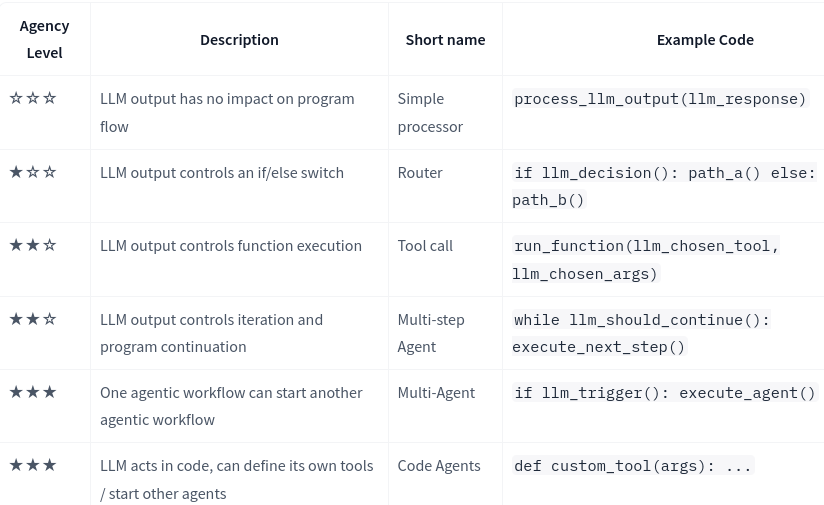
\includegraphics[width=\textwidth]{agent-levels.png}
    		\caption{\url{https://huggingface.co/docs/smolagents/en/conceptual_guides/intro_agents}}
    	\end{figure}
    \end{frame}
    
    
    \section{Agent-to-Agent Interaction}
  
    \subsection{Single-Agent vs. Multi-Agent}
    
    \begin{frame}
    	\sectionpage
    	\subsectionpage
    \end{frame}
    
    \subsection{Orchestrating Interaction}
    
    \begin{frame}
    	\sectionpage
    	\subsectionpage
    \end{frame}
    
    \subsection{What do we actually need?}
    
    \begin{frame}
    	\sectionpage
    	\subsectionpage
    \end{frame}

\end{document}
